\documentclass[10pt,a4paper]{article}
\usepackage[utf8]{inputenc}
\usepackage{amsmath}
\usepackage{amsfonts}
\usepackage{amssymb}
\usepackage{graphicx}

\title{Snowmass  H$\gamma\gamma$ and HZ$\gamma$ CP studies}
\author{S. Kyriacou}



\begin{document}

\maketitle

\section{POIs and relations}

This is a study of a pp collider sensitivity to anomalous CP  $HZ\gamma$ and $H\gamma\gamma$ couplings. 
The couplings of interest are $a_{3}^{\gamma\gamma}$,$a_{2}^{\gamma\gamma}$,$a_{3}^{Z\gamma}$, and$a_{2}^{Z\gamma}$. 
In the AC analysis using the mass eigenstate basis, we usually perform a measurement of the fractional cross-section contributions of each AC to the total cross-section, rather than a direct coupling strength measurement. 

For the Snowmass studies, we want to define collider independent quantities which we can use to estimate constraints and compare then sensitivity between the different machines. For this reason we define as parameters of interest the quantities defined in eq. \ref{eq:fggnew}: 

\begin{equation} \label{eq:fggnew}
\begin{aligned}
f^{\gamma\gamma} &= fa3^{\gamma\gamma} + fa2^{\gamma\gamma} \\
f^{\gamma\gamma}_{CP} &= \frac{fa3^{\gamma\gamma}}{\lvert fa3^{\gamma\gamma} \rvert + \lvert fa2^{\gamma\gamma} \rvert}
\end{aligned}
\end{equation}

and 

\begin{equation} \label{eq:fZgnew}
\begin{aligned}
f_{Z\gamma} &= fa3Z\gamma + fa2Z\gamma \\
f_{Z\gamma\gamma}^{CP} &= \frac{fa3Z\gamma}{\lvert fa3Z\gamma \rvert + \lvert fa2Z\gamma \rvert}
\end{aligned}
\end{equation}


In the physics model when scanning for fai3 we set it as the primary POI (for example fa3) and then the rest of the ac -fais are deined with relation to that, using auxiliary free parameters (what is named fai\textunderscore relative in the physics model) for the definitions. 
So for an fa3 scan we have 4 free parameters: 
\\
\\
fai2, fai1relative, fai3relative, fai4relative
\\
\\
Then the parameters: fai1, fai3 and fai4 
are dependent parameters and functions of the free parameters listed above\footnote{What we map as the AC corresponding to the fai3,fai2 etc is completetly arbitrary and is a choise one defines in the physics model. For equations \ref{eq:fggnew} fai3 corresponds to $a3^{\gamma\gamma}$, fai2 to $a2^{\gamma\gamma}$ and to complete the choice, fai4  corresponds to $a2^{Z\gamma}$ and fai1 to $a3^{Z\gamma}$. Another notation issue is that $fai[2-4]=fa[2-4]$ while $fa1$ corresponds to SM while $fai1$ corresponds to the AC that is left from the previous definitions, in this case $a3^{Z\gamma}$. Very important is the fact that the fai[1-4] are tied to the gis thus ou can not do a scan where fai4 is identified as $f_{\gamma\gamma}$ or other new parameter.},for example: 

\begin{equation}\label{eq:usualdep}
\begin{align}
fai3 &= (1-|fai2|)fai3relative\\
fai4 &= (1-|fai3| -|fai2| )fai4relative\\
fai1 &= (1-|fai3| -|fai4| - |fai2| )fai1relative
\end{align}
\end{equation}
 
  
  
The anomalous couplings strengths (gi) multiplying the templates for physics processes in the likelihood are defined as fuctnions of the fais, where the xsection ratio information is also inserted. This has been the modus operanti for all our previous fai work. 


One can then use $f_{\gamma\gamma}$ or $f_{\gamma\gamma}^{cp}$, or even both of them as the free parameters and then define the depended parameters fai as functions of the new parameters rather than the orignal ones. 
One case is using only  $f_{\gamma\gamma}^{cp}$ as a free parameter and replacing fai3relative, then eq. \ref{eq:usualdep} are modified as:  


\begin{equation}\label{eq:newdepfcp}
\begin{align}
fai3 &= \frac{f_{\gamma\gamma}^{CP} |fai2|}{(1 -f_{\gamma\gamma}^{CP})}   &\mathrm{ for } &f_{\gamma\gamma}^{CP} > 0  \\
     &= \frac{f_{\gamma\gamma}^{CP} |fai2|}{(1 + f_{\gamma\gamma}^{CP})}  &\mathrm{ for } &f_{\gamma\gamma}^{CP} < 0  \\
fai4 &= (1-|fai3| -|fai2| )fai4relative\\
fai1 &= (1-|fai3| -|fai4| - |fai2| )fai1relative
\end{align}
\end{equation}
with the bifurcation in the fai3 function caused by the absolute value of fai3 in the denominator of the $f_{\gamma\gamma}^{CP}$ definition. The other condition here is the sign of fai2 which changes in the denominator
Another case is choosing $f_{\gamma\gamma}$ as the free parameter to replace fai3relative
In this case the relations are more trivial: 

\begin{equation}\label{eq:newdepfgg}
\begin{align}
fai3 &= f_{\gamma\gamma} -  fai2\\
fai4 &= (1-|fai3| -|fai2| )fai4relative\\
fai1 &= (1-|fai3| -|fai4| - |fai2| )fai1relative
\end{align}
\end{equation}

The picture is similar for the $HZ\gamma$ couplings.
The absolutes in the denominator of  $f_{\gamma\gamma}^{CP}$ do not allow for an easy simultaneous definition of the $f_{\gamma\gamma}^{CP}$ and $f_{\gamma\gamma}$ as free parameters in a single setup. 

As a test for the validity of these transformations, we perform a scan of $fa2\gamma\gamma$ with the relations in eq.  \ref{eq:usualdep} and compare it to a scan where  $f_{\gamma\gamma}^{CP}$ has replace fai3relative as a free parameter, namely eq. \ref{eq:newdepfcp}. The test can be seen in fig. . The lines overlap thus validating our procedure. 

\begin{figure}[t]
\centering
\includegraphics[width=0.45\textwidth]{./output_fa2gg_test.pdf}
\caption{Projected scans for $fa2\gamma\gamma$ with the original and new dependency definitions that should not affect $fa2\gamma\gamma$. The scans are identical validating our method. }
\label{fig:fcgg}
\end{figure}


\section{Considering SM}

The definitions in eq. \ref{eq:fggnew} are probematic for SM in the absence of any kind of loop effects or anomalous couplings. Namely $f_{\gamma\gamma}^{CP}$ is undefined for $a3^{\gamma\gamma} = 0$ and $a2^{\gamma\gamma} = 0$. One can study the CP component though in the presensece of NLO EW effects that can be modeled by a small a2 contribution. The value for $a2^{\gamma\gamma}$ that can reproduce the $H\rightarrow \gamma\gamma$ decay is
\begin{equation} 
a_{2}^{\gamma\gamma,SM} = 0.00423 
\end{equation}
The corresponding fai2 value for  $a2^{\gamma\gamma,SM}$ is\footnote{The value and calculation has been cross-checked between the physics model implementation and the definition calculation using Table3 from our virtual photons pheno paper.  } 
 
\begin{equation}
 f_{a2}^{\gamma\gamma,SM} = 0.00631365
 \end{equation}
 
 
Thus the corresponding SM values for the POIs of eq. \ref{eq:fggnew} are \\


 $f^{\gamma\gamma,SM} = f_{a2}^{\gamma\gamma,SM}$ and $f^{\gamma\gamma,SM}_{CP} = 0$  . 

The SM values for the $HZ\gamma$ POIs are 0. 







\section{Results}

We test the sensitivity of a $H\rightarrow 4l$ analysis in a pp collider to $f_{\gamma\gamma}$ and $f_{\gamma\gamma}^{cp}$ with a projected integrated luminocity 3000$ab^{-1}$. The SM hypothesis, used to generate the MC toys,  includes the NLO EW effects and the values that correspond to the POIs are listed in the previous section. 
\\
We introduce  $f_{\gamma\gamma}^{CP}$ as a new POI and use relations in \ref{eq:newdepfcp} to define the dependent POIs $(fai3,fai2,fai1)$ and scan for the new parameter. In a different setup we introduce $f_{\gamma\gamma}$ as the new POI and use the relations in \ref{eq:newdepfgg} to define the dependent parameters. Following this we scan for  $f_{\gamma\gamma}$. In fig. \ref{fig:fcgg} the results for the scans of the $f_{\gamma\gamma}$ and $f_{\gamma\gamma}^{cp}$ are presented. 

A similar procedure is followed and we obtain scans for $f_{Z\gamma}$ and $f_{Z\gamma}^{cp}$, the results of which are presented in fig. \ref{fig:fzgg}. 




\begin{figure}[t]
\centering
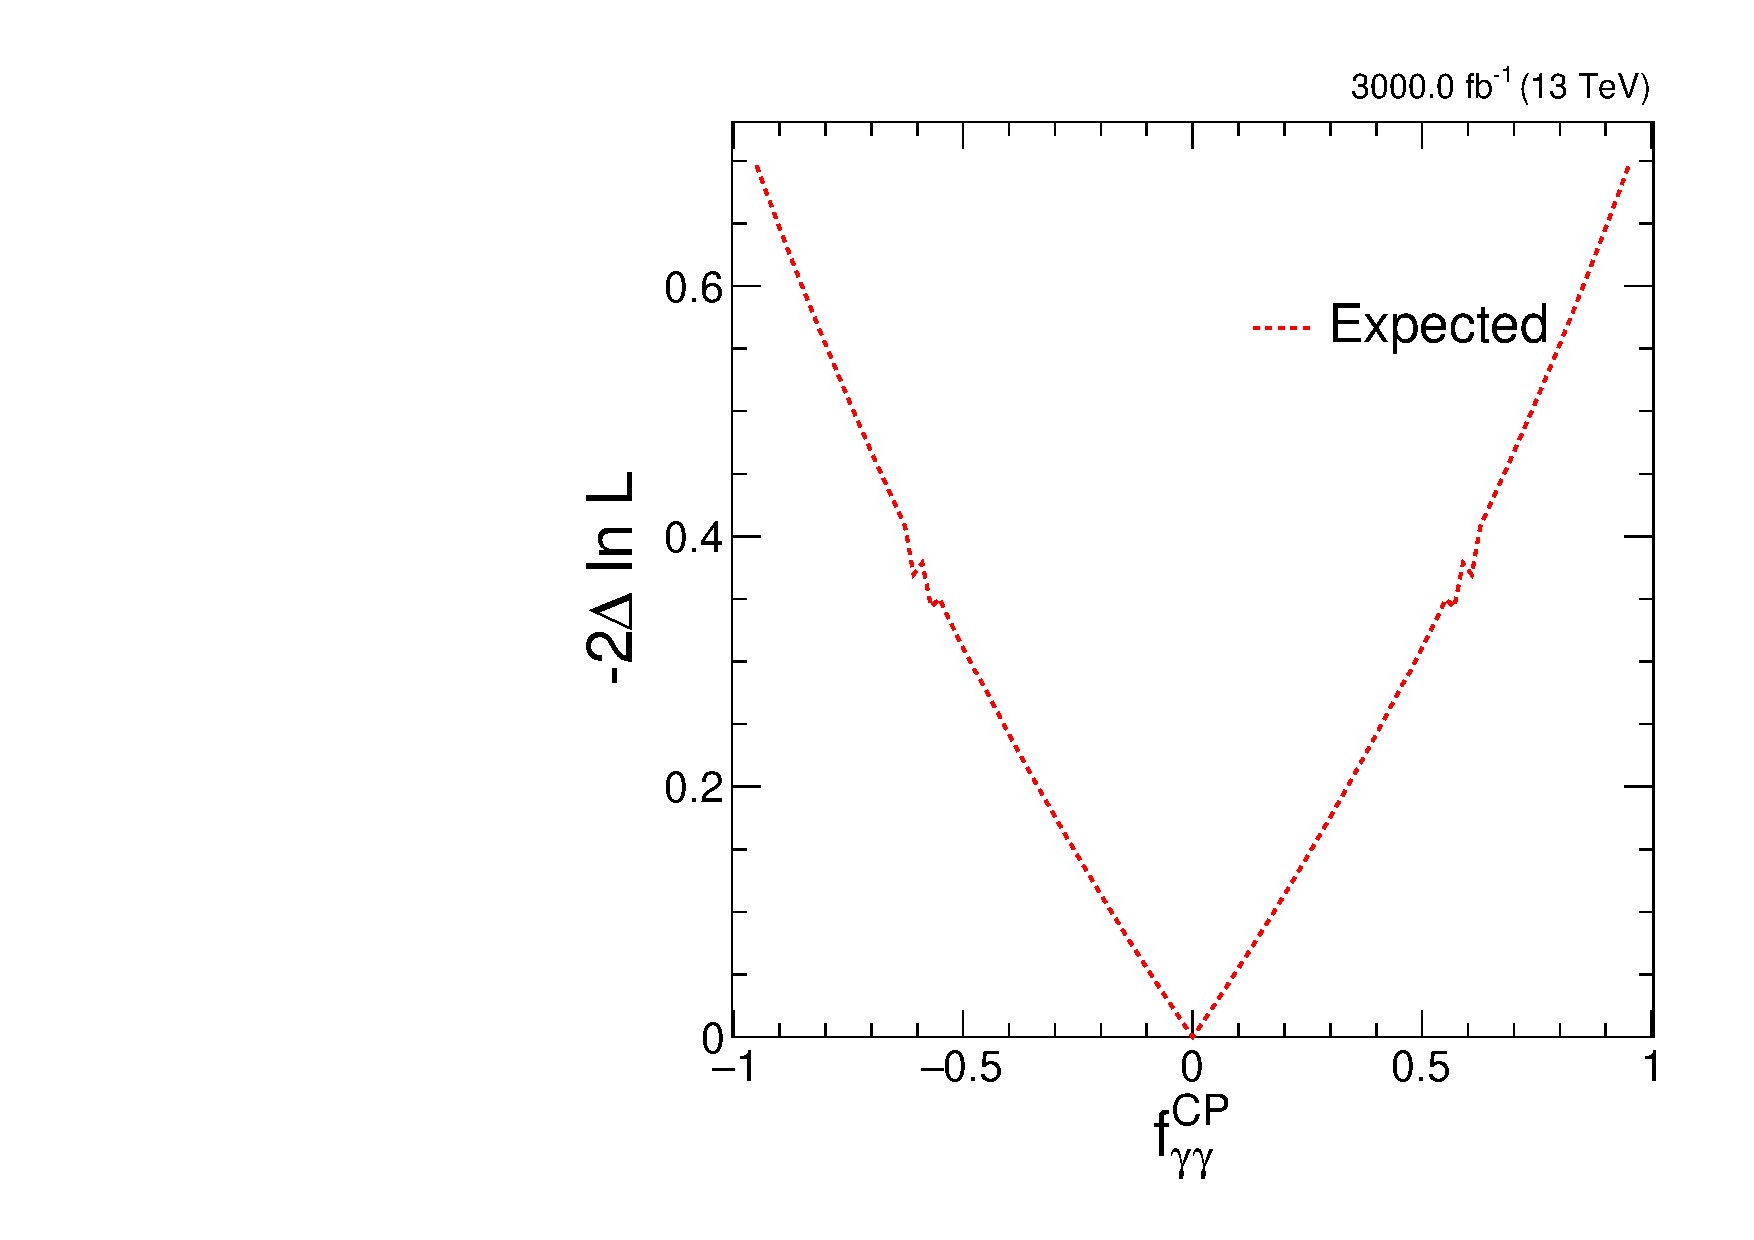
\includegraphics[width=0.45\textwidth]{./output_fggcp.pdf}
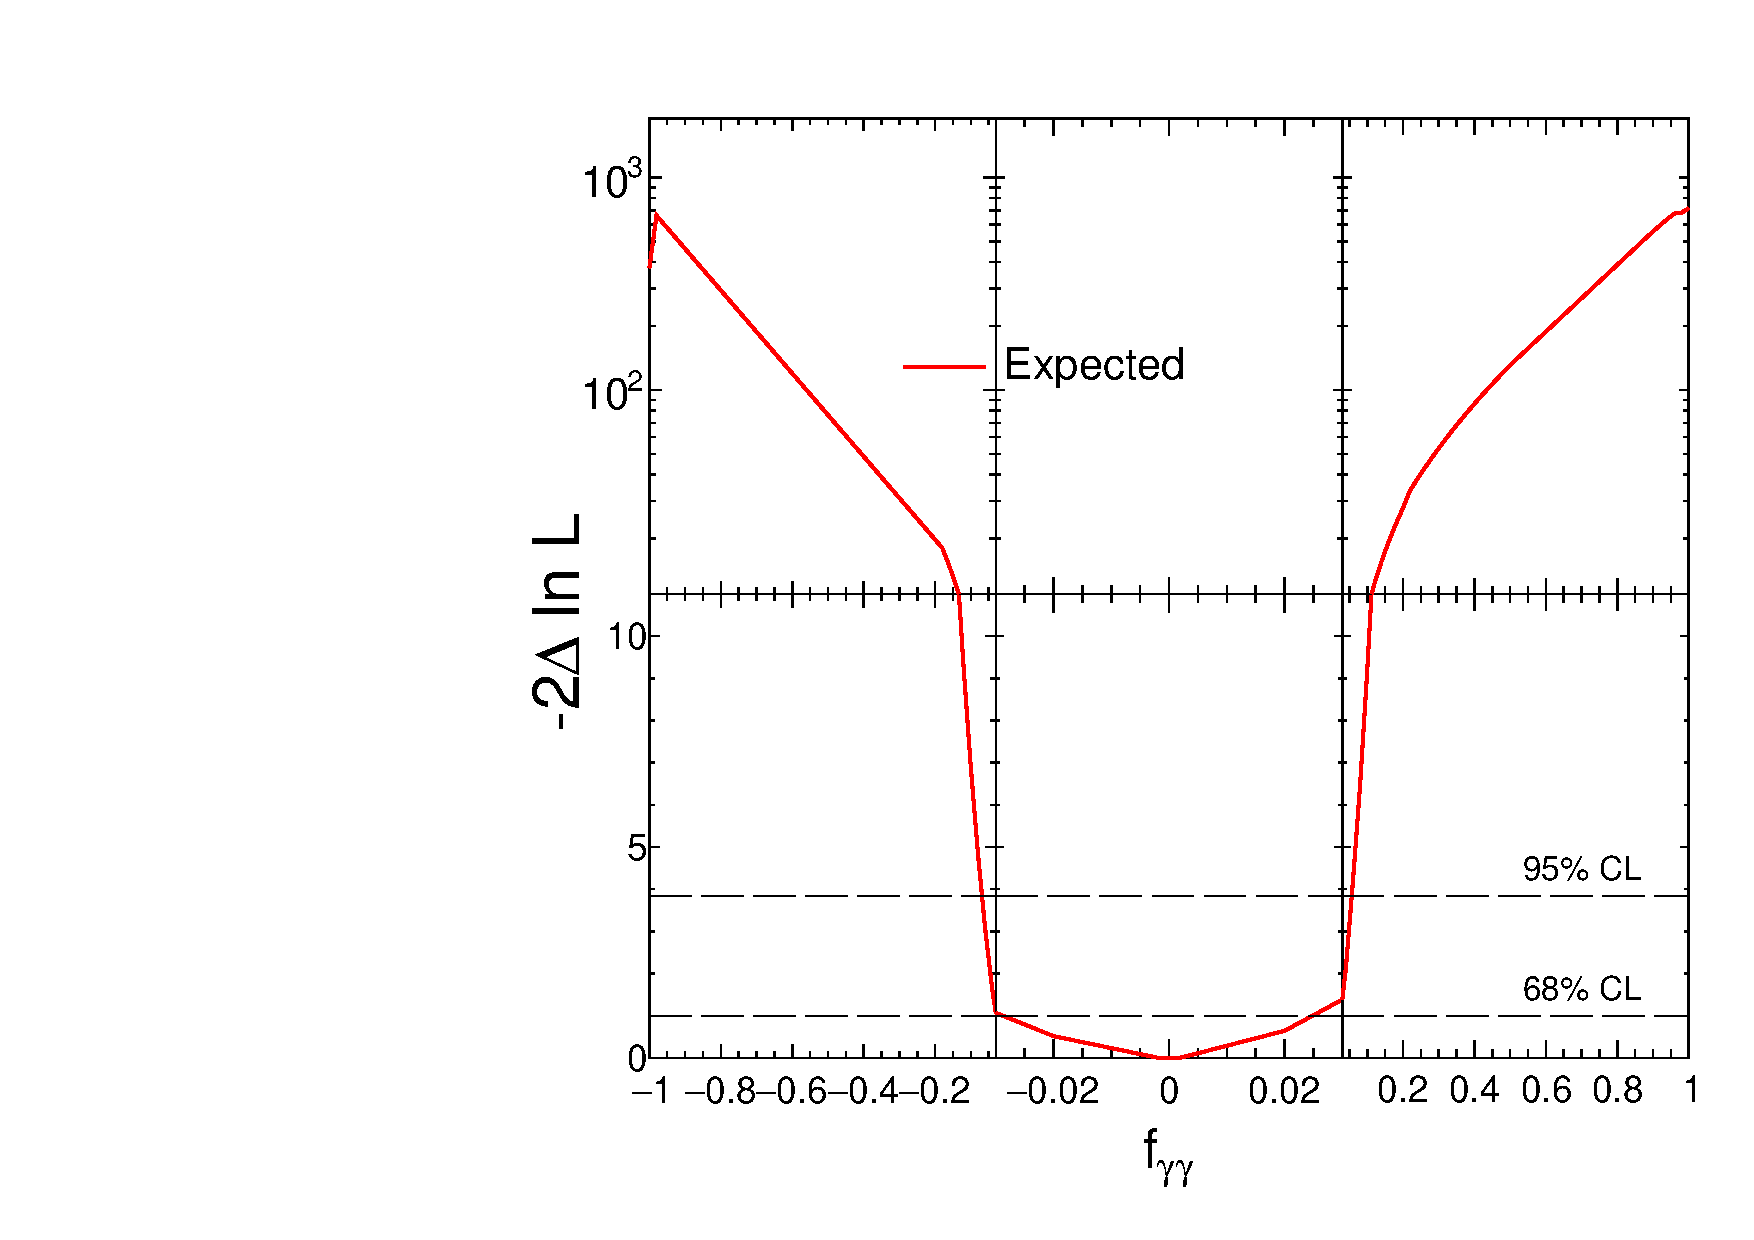
\includegraphics[width=0.45\textwidth]{./output_fgg.pdf}
\caption{Projected scans for $f_{\gamma\gamma}^{CP}$ (left) and $f_{\gamma\gamma}$(right)}
\label{fig:fcgg}
\end{figure}



\begin{figure}[t]
\centering
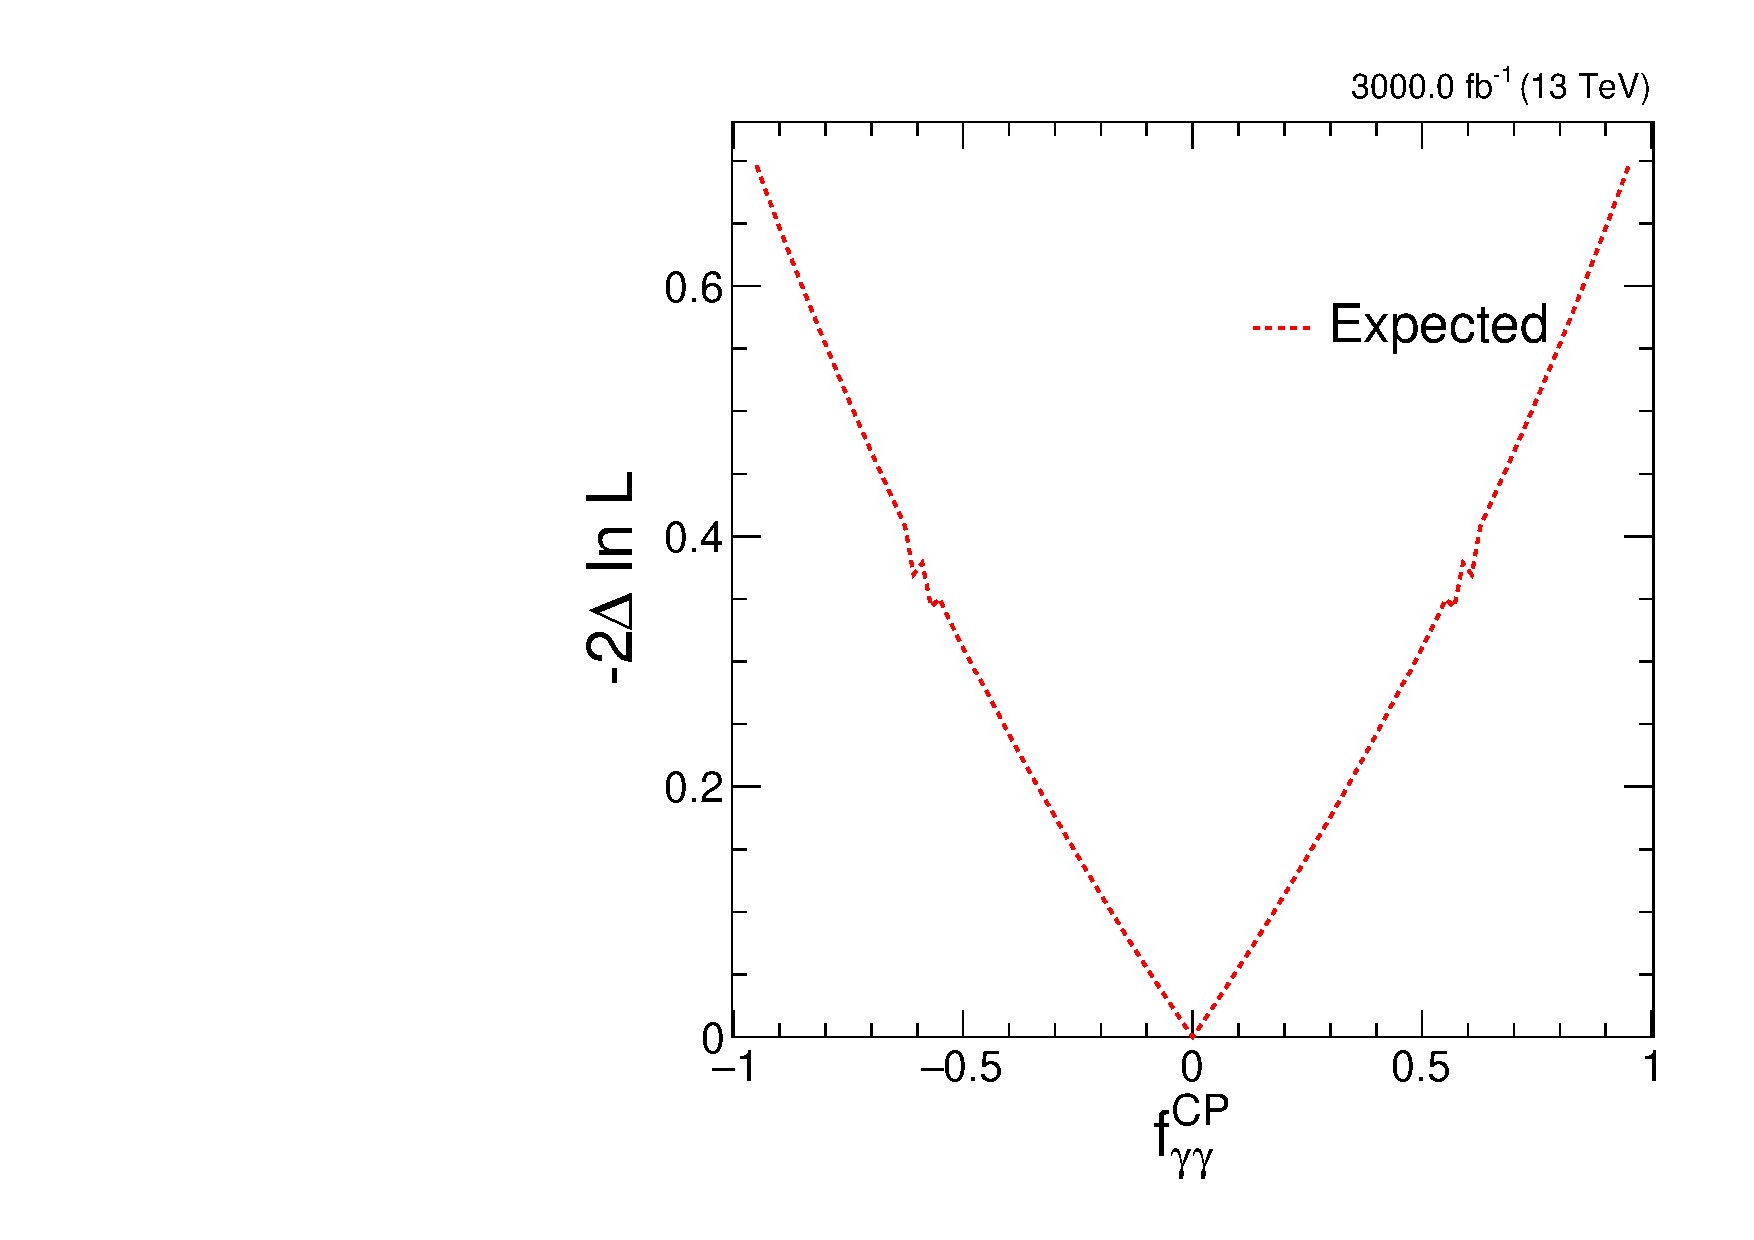
\includegraphics[width=0.45\textwidth]{./output_fggcp.pdf}
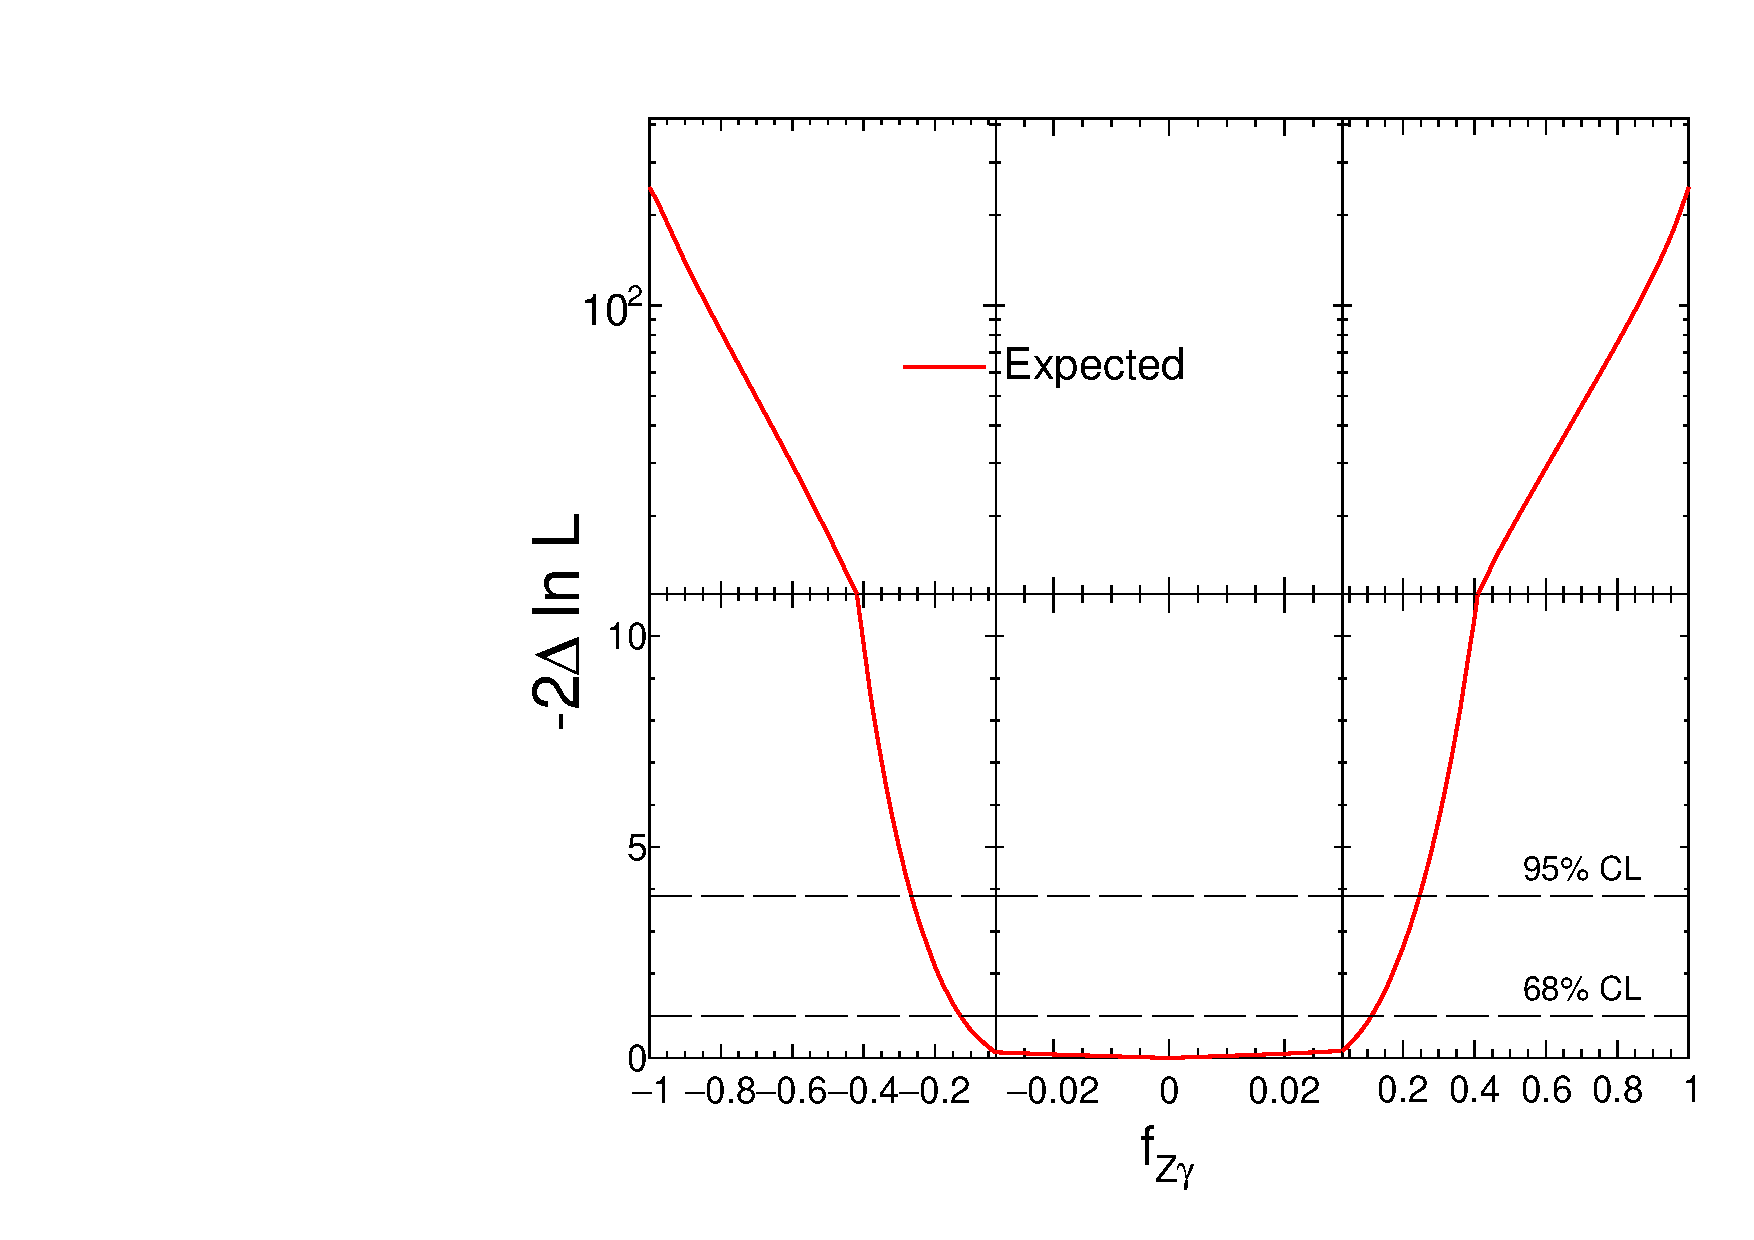
\includegraphics[width=0.45\textwidth]{./output_fzg.pdf}
\caption{Projected scans for $f_{Z\gamma}^{CP}$ (left) and $f_{Z\gamma}$(right)}
\label{fig:fzgg}
\end{figure}




\section{Relations for simultaneous $f^{\gamma\gamma}$ and $f^{\gamma\gamma}_{CP}$ scans }


fai3 has the sign of $f_{\gamma\gamma}^{CP}$ based on def in eq. \ref{eq:fggnew}. 
The problem arrizes that one can not uniquely define the sign of fa2 from the signs of $f_{\gamma\gamma}^{CP}$ and  $f_{\gamma\gamma}$. There are subcases that the sign can be determined using the signs of the new parameters only such as: 
\begin{equation}
\begin{align}
sign(fai3) &= sign(f_{\gamma\gamma}^{CP}) &\mathrm{always} \\
sign(fai2) &> 0 &\mathrm{if}\, f_{\gamma\gamma} > 0  \,&\mathrm{and }\, f_{\gamma\gamma}^{CP} < 0 \\
sign(fai2) &< 0 &\mathrm{if}\, f_{\gamma\gamma} < 0  \,&\mathrm{and }\, f_{\gamma\gamma}^{CP} > 0 \\
sign(fai2) &\,\mathrm{ undefined}  &\mathrm{if }\, f_{\gamma\gamma} > 0  \,&\mathrm{and }\, f_{\gamma\gamma}^{CP} > 0 \\
sign(fai2) &\,\mathrm{ undefined}  &\mathrm{if }\, f_{\gamma\gamma} < 0  \,&\mathrm{and }\, f_{\gamma\gamma}^{CP} < 0 
\end{align}\label{eq:signs}
\end{equation}

Nevertheless we can study some subcases


\begin{equation}\label{eq:newdepfggfcp}
\begin{align}
fai3 &= f_{\gamma\gamma}^{CP}(|fai3| +|fai2|) & \\
fai3 &= f_{\gamma\gamma}^{CP}(fai3 +|fai2|) &\mathrm{assuming } f_{\gamma\gamma}^{CP} > 0 & \\
fai3 &= \frac{f_{\gamma\gamma}^{CP}|fai2|}{1-f_{\gamma\gamma}^{CP}} &
\end{align}
\end{equation}

Thus continuing down this path we have where $f_{\gamma\gamma}^{CP} > 0$: 


\begin{equation}
\begin{align}
fai2 &= f_{\gamma\gamma} - fai3 \\
fai2 &= f_{\gamma\gamma}  - \frac{f_{\gamma\gamma}^{CP}|fai2|}{1-f_{\gamma\gamma}^{CP}}  
\end{align}\label{eq:newdepfggfcpfa2}
\end{equation}



\section{Alternative definition of $f^{\gamma\gamma}$, $f^{Z\gamma}$   and results }


We are change the definition of $f_{\gamma\gamma}$ as but retain what we consider as $f_{\gamma\gamma}^{CP}$: 
\begin{equation} \label{eq:fggnewdef}
\begin{aligned}
f^{\gamma\gamma} &= |f_{a3}^{\gamma\gamma}| + |f_{a2}^{\gamma\gamma}| \\
f^{\gamma\gamma}_{CP} &= \frac{f_{a3}^{\gamma\gamma}}{\lvert f_{a3}^{\gamma\gamma} \rvert + \lvert f_{a2}^{\gamma\gamma} \rvert}
\end{aligned}
\end{equation}

This setup allows for an easy simultaneous consideration of the two parameters as the free POIs. The dependency relations are thus altered as well to become in this case: 


\begin{equation}\label{eq:newdepfcp}
\begin{align}
fai3 &= f_{\gamma\gamma}f_{\gamma\gamma}^{CP}\\
fai2 &= f_{\gamma\gamma} - |fai3|  \\
fai4 &= (1-|fai3| -|fai2| )fai4relative\\
fai1 &= (1-|fai3| -|fai4| - |fai2| )fai1relative
\end{align}
\end{equation}

Similarly we can define for the $HZ\gamma$ couplings the relations: 


\begin{equation} \label{eq:fZgnewdef}
\begin{aligned}
f^{Z\gamma} &= |f_{a3}^{Z\gamma}| + |f_{a2}^{Z\gamma}| \\
f^{Z\gamma}_{CP} &= \frac{f_{a3}^{Z\gamma}}{\lvert f_{a3}^{Z\gamma} \rvert + \lvert f_{a2}^{Z\gamma} \rvert}
\end{aligned}
\end{equation}



What SM corresponds in this new definition does not change from the previous setups, namely 
$f_{\gamma\gamma} = fai2^{SM}$ and with all other POIs from eq. \ref{eq:fggnewdef} and \ref{eq:fZgnewdef} to be zero. We encode this definition and proceed to perform simultaneous scans of the two POIs. The results of can be seen in fig. \ref{fig:2D} for a 2D scan and corresponding 1D scans for the two parameters can are presented in in fig. \ref{fig:1D_fgg_fggcp}. Similar relationship, setting as free parameters $f_{\gamma\gamma}$, $f_{Z\gamma}$ and $f^{Z\gamma}_{CP}$ are presented in \ref{fig:1D_fzg_fzgcp}. In this case the setting of $f_{\gamma\gamma}$ as a free parameter is necessary to set the SM value for the toy generation. 


\begin{figure}[t]
\centering
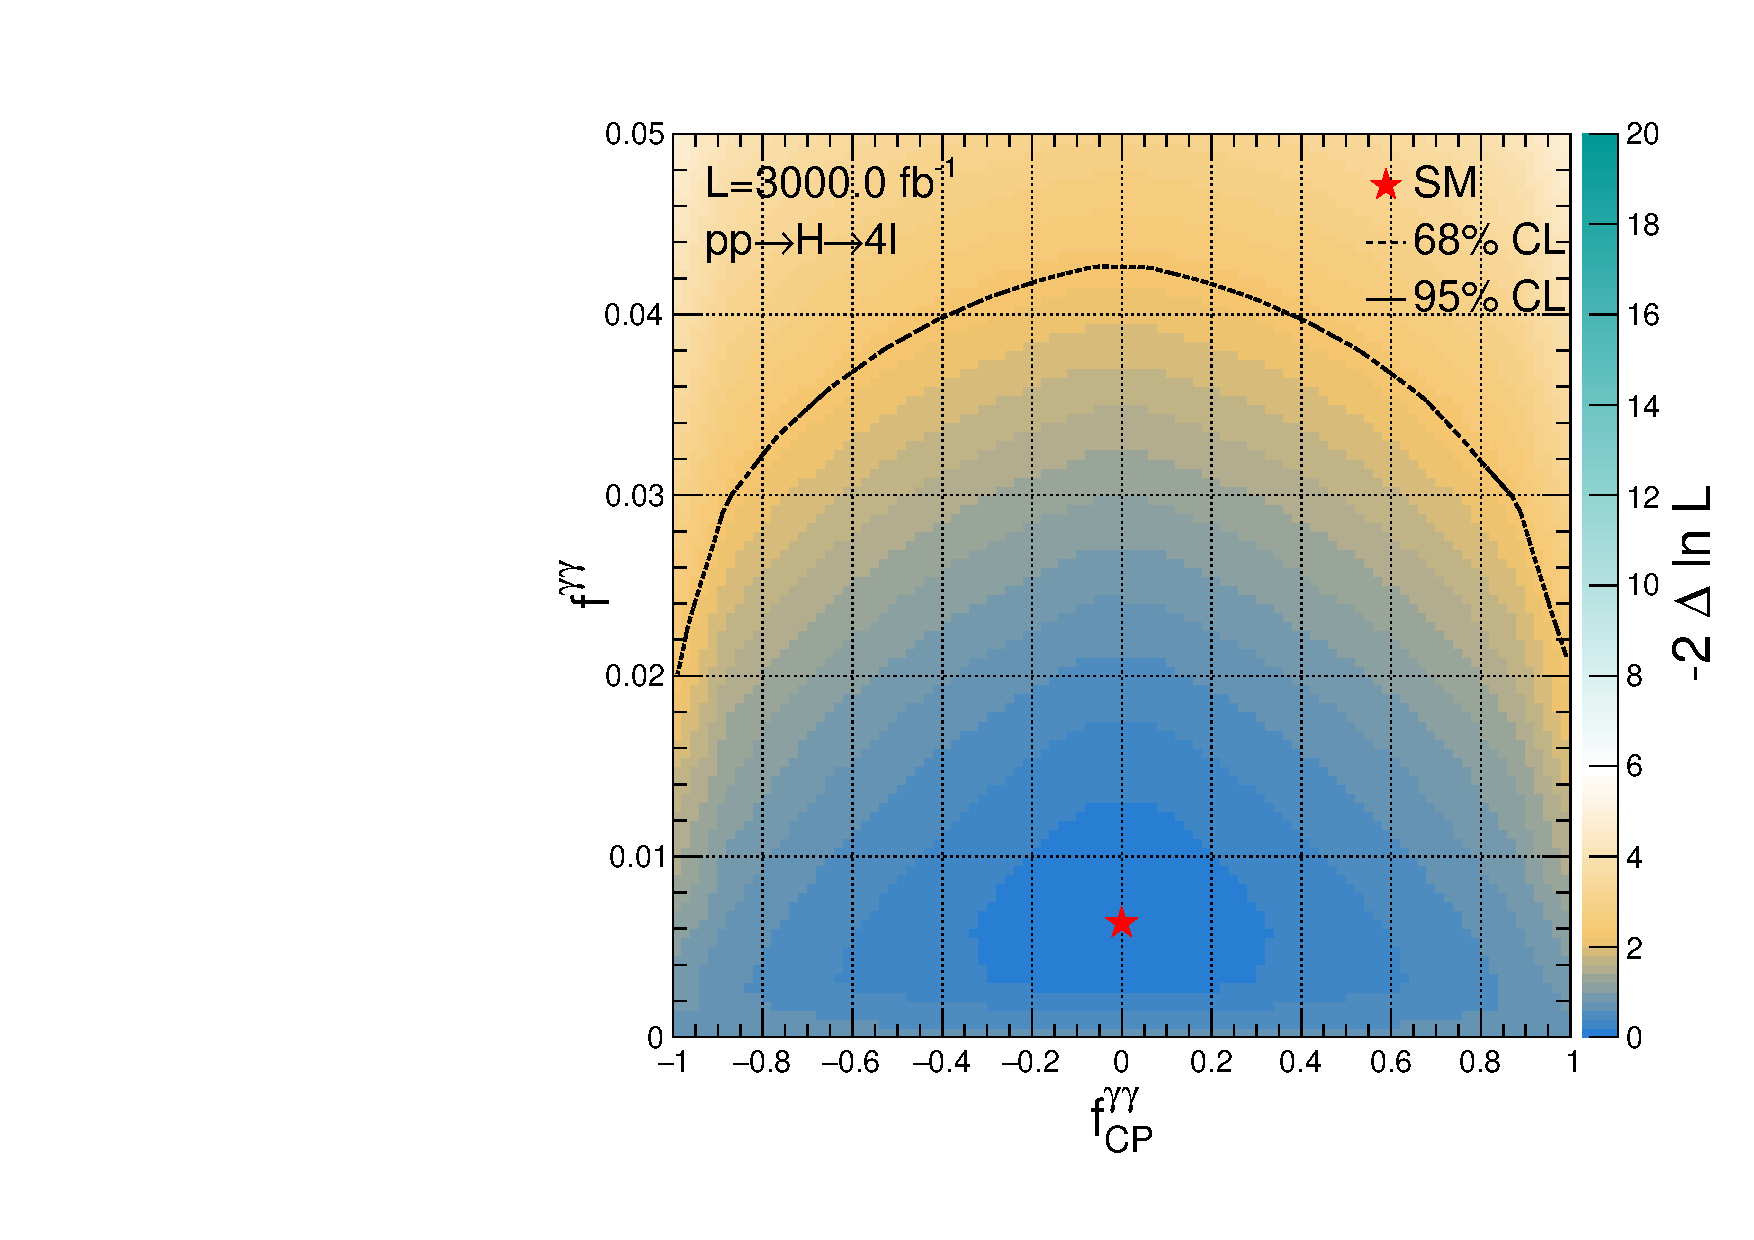
\includegraphics[width=0.8\textwidth]{./2D/2D_fgg_fggcp.pdf}
\caption{A two dimensional scan of  $f_{\gamma\gamma}^{CP}$ and $f_{\gamma\gamma}$ with the alternative definition}
\label{fig:2D}
\end{figure}



\begin{figure}[t]
\centering
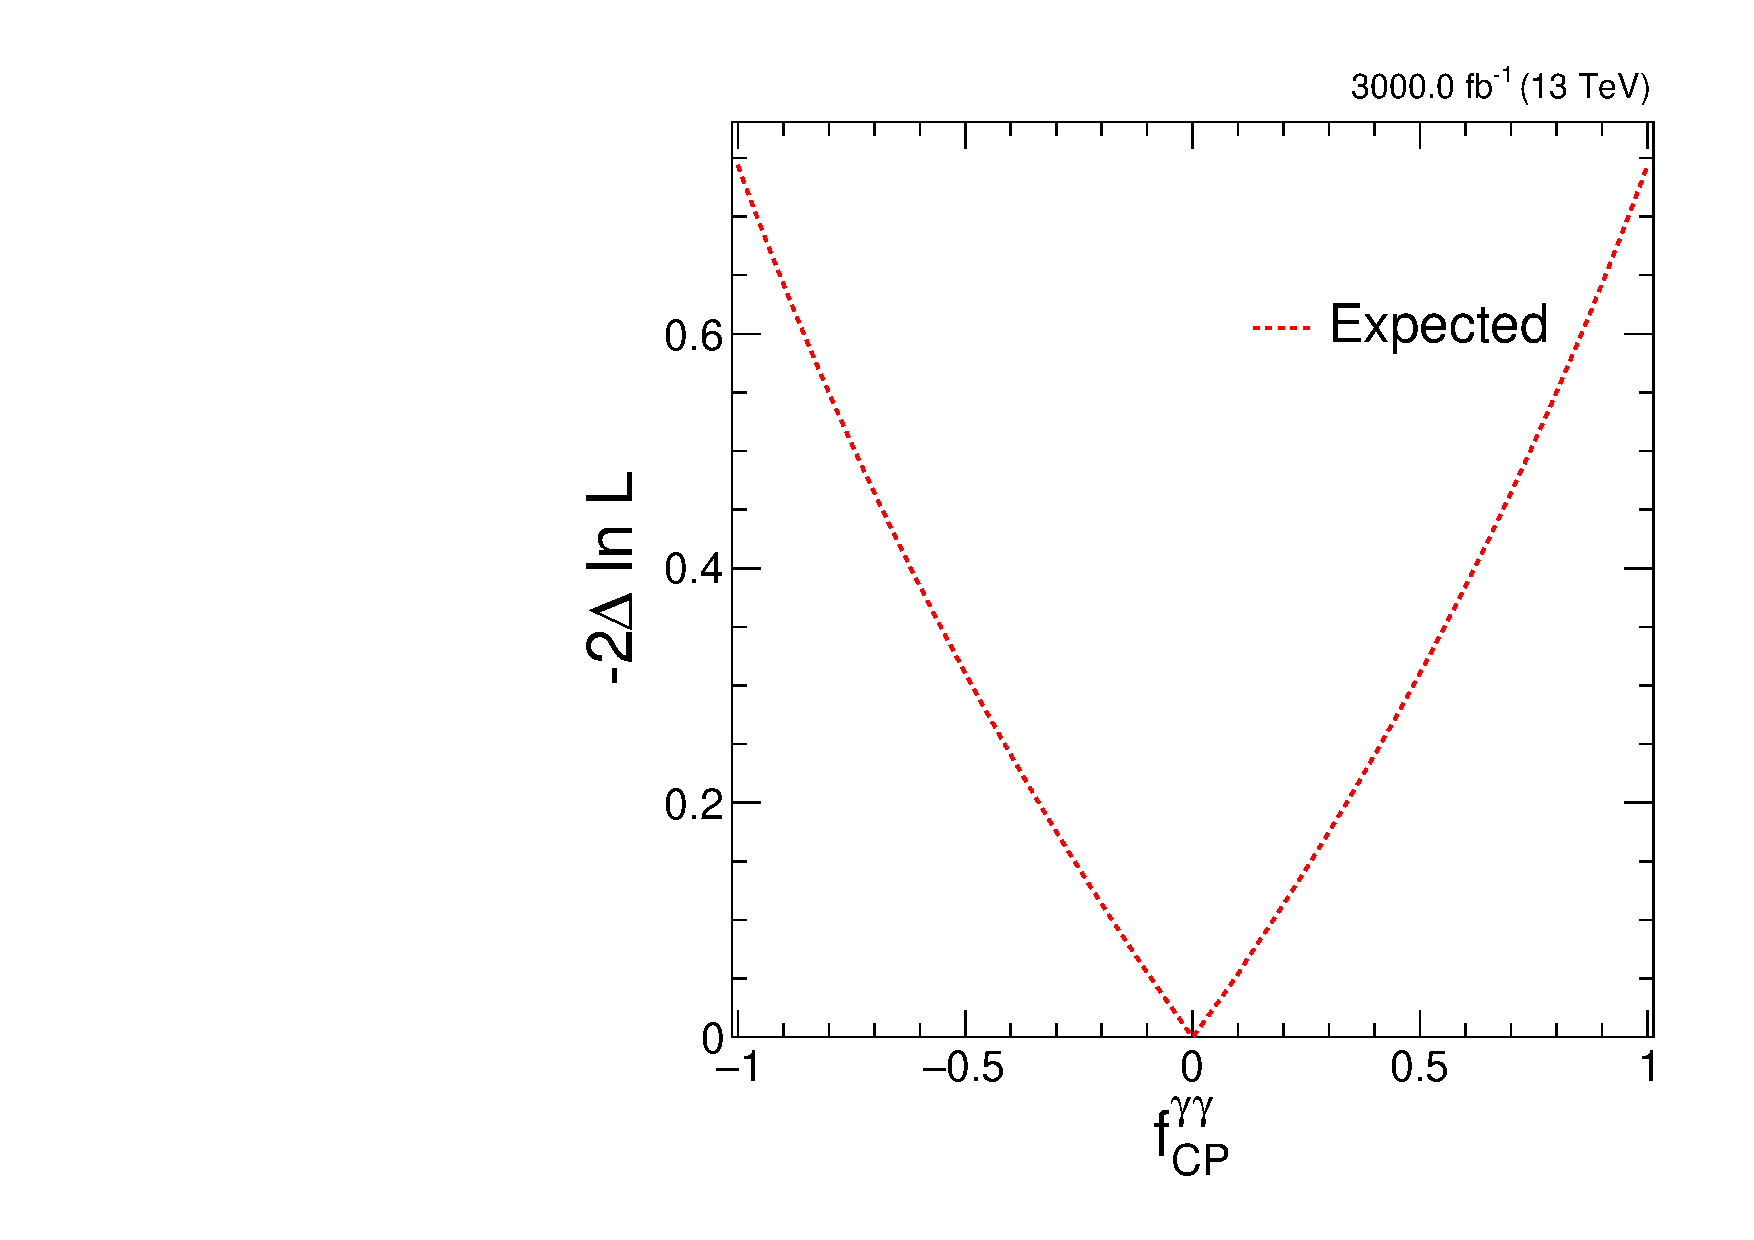
\includegraphics[width=0.45\textwidth]{./output_alt_fggcp.pdf}
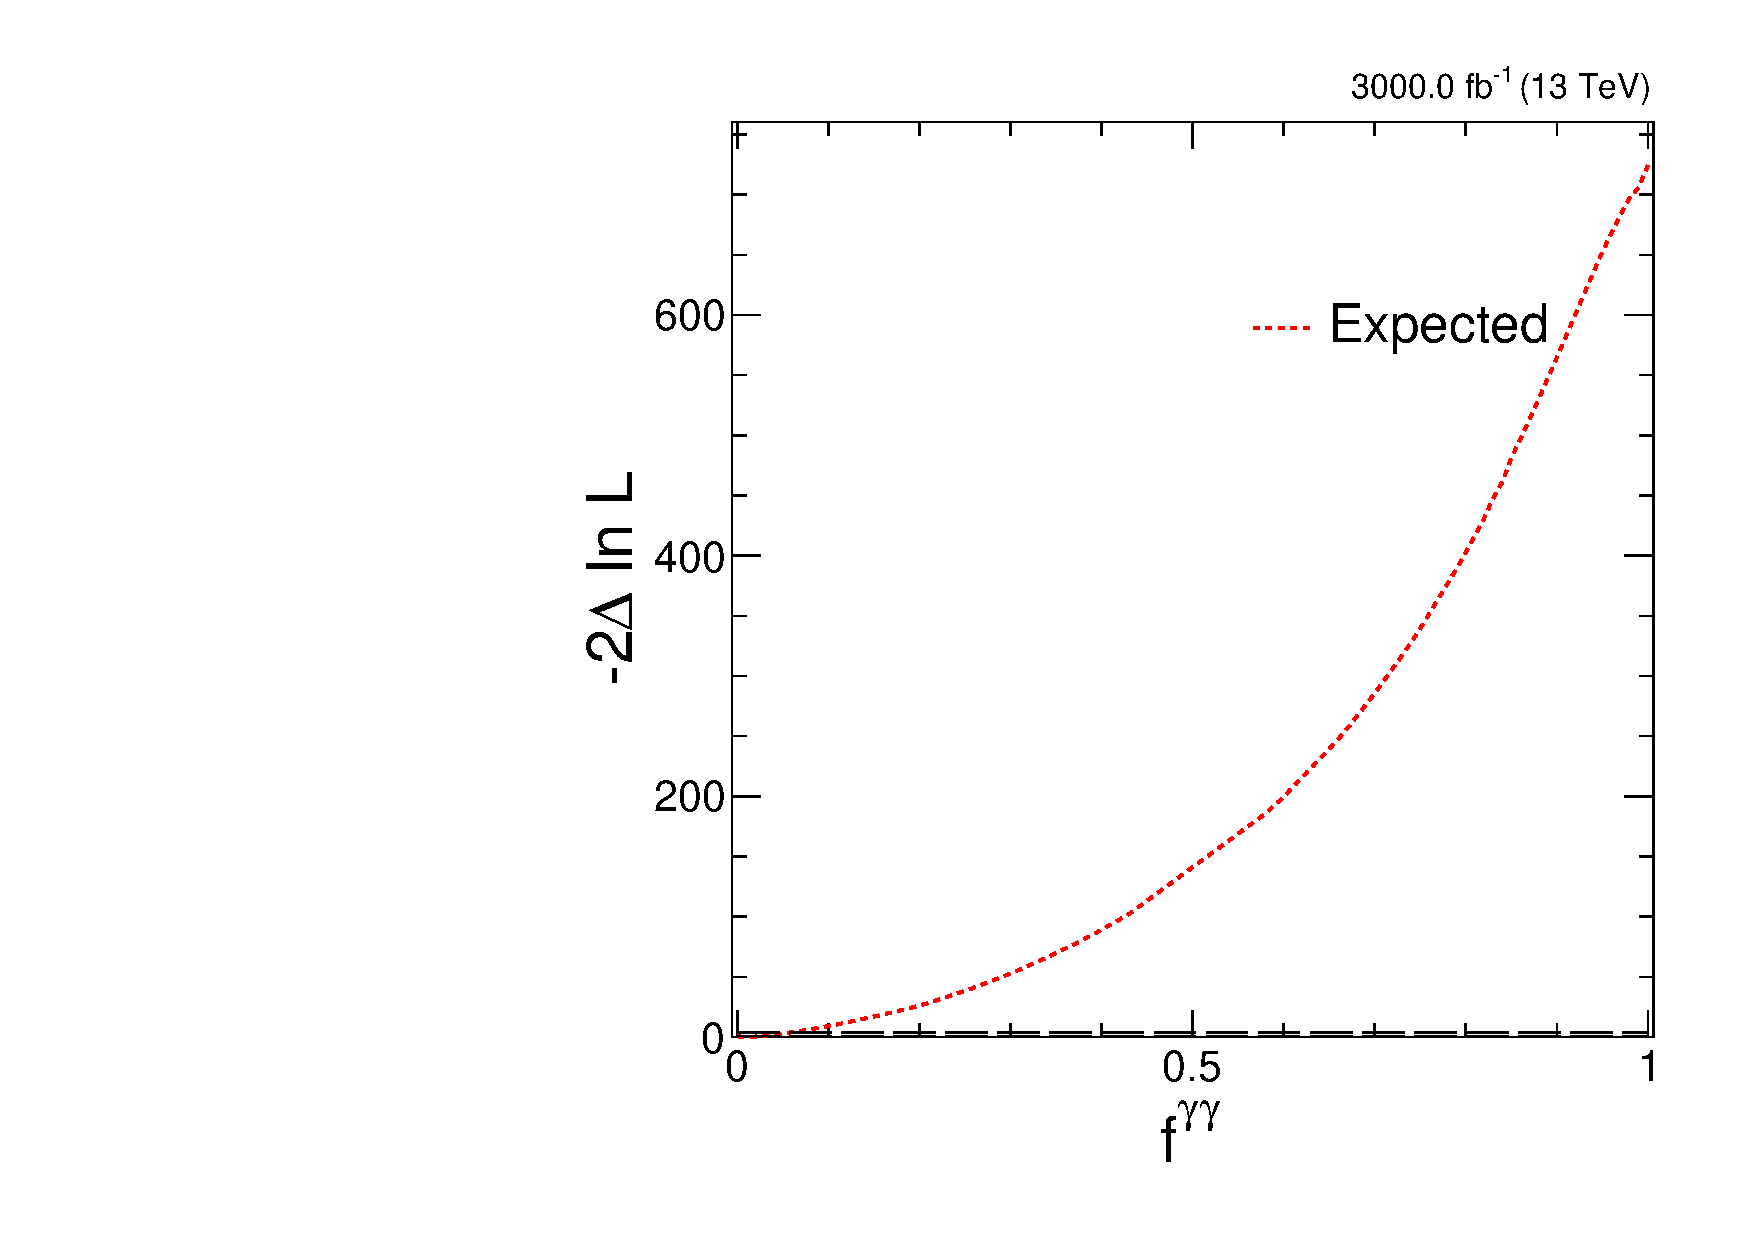
\includegraphics[width=0.45\textwidth]{./output_alt_fgg.pdf}
\caption{1D scans for $f_{\gamma\gamma}^{CP}$(right) and $f_{\gamma\gamma}$(left) with the alternative definition}
\label{fig:_fgg_fggcp}
\end{figure}


\begin{figure}[t]
\centering
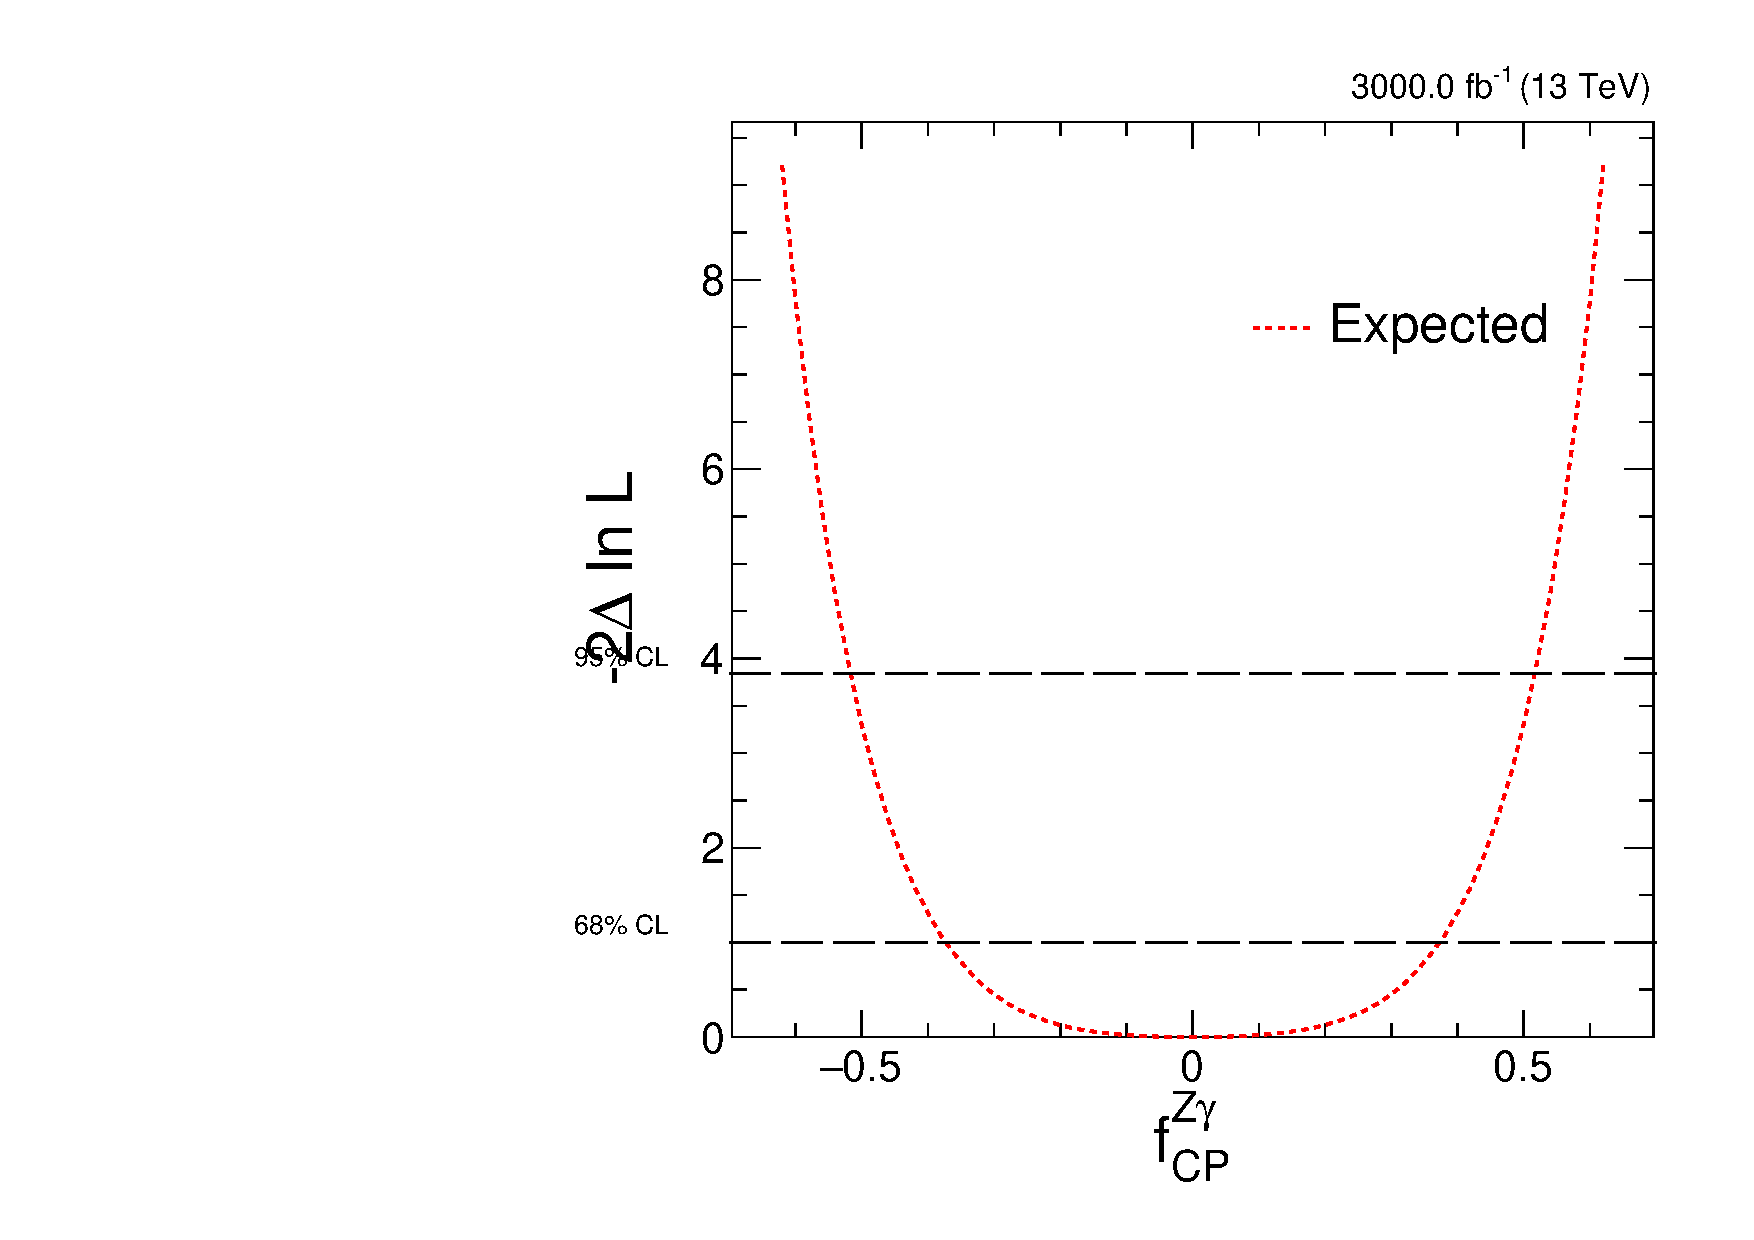
\includegraphics[width=0.45\textwidth]{./output_alt_fzgcp.pdf}
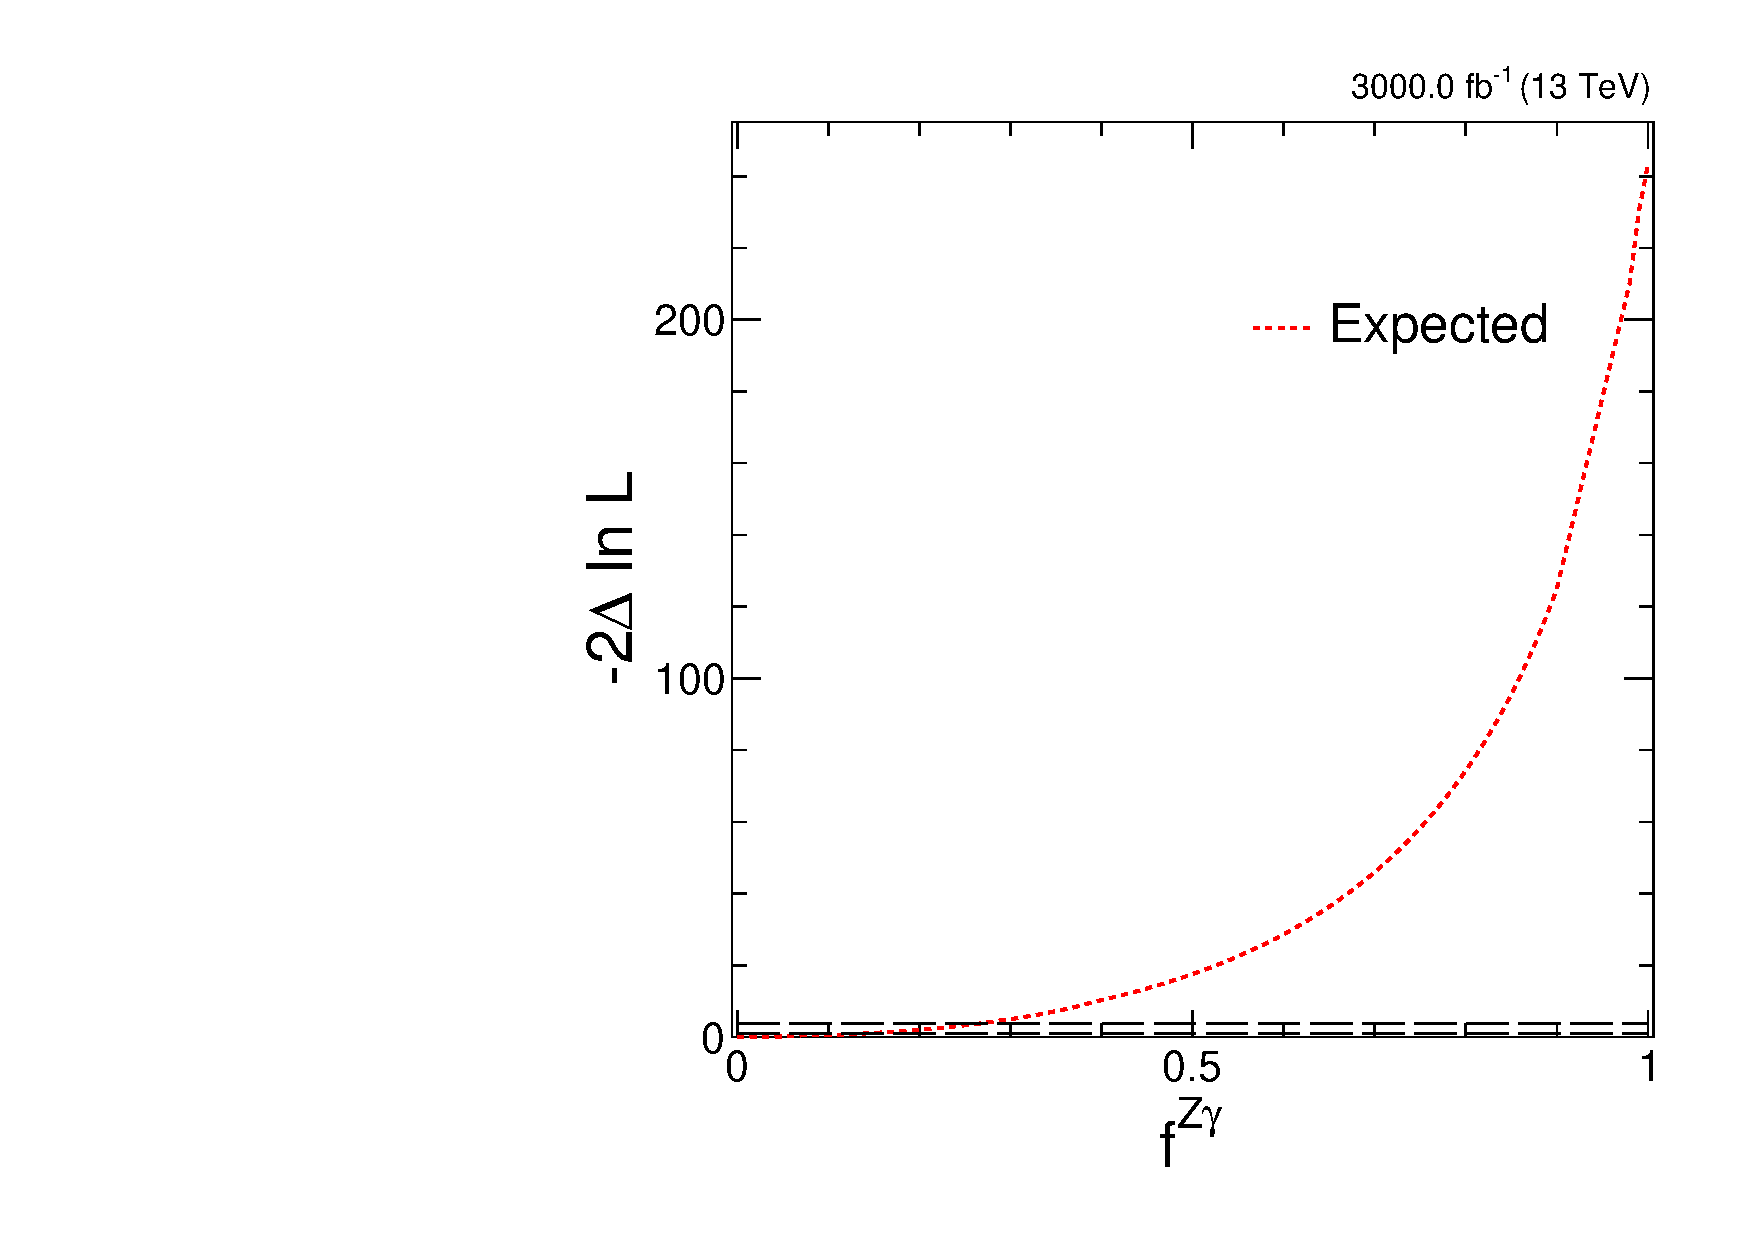
\includegraphics[width=0.45\textwidth]{./output_alt_fzg.pdf}
\caption{1D scans for $f^{Z\gamma}^{CP}$(left) and $f^{Z\gamma}$(right) with the alternative definition}
\label{fig:_fzg_fzgcp}
\end{figure}






\\
\\
\\






\end{document}